\documentclass[
headings=optiontohead,              % allows double headers
12pt,                               % fontsize 
DIV=13,                             % koma script diveider amount. tells koma how much of the site can be written to
twoside=false,                      % if set to true, automatically formats as book style with different left and right pages
open=right,                         % starting page on twosided texts 
BCOR=10mm,                          % correction that accounts for the center of the pages being glued in
toc=bibliographynumbered            % bibliography gets a number and is listed in the table of contents
]{scrreport}

\usepackage[utf8]{inputenc}                     % correct encoding of output, technically not needed anymore
\usepackage[T1]{fontenc}                        % correct encoding of output, technically not needed anymore
\usepackage[english]{babel}                     % font that supports English
\usepackage{upgreek}                            % non-cursive Greek letters
\usepackage[stretch=10,shrink=10,protrusion=true,expansion=true,final]{microtype} % prettier block format
\usepackage{hyperref}                           % links for everything
\usepackage{color}                              % allows for setting in different colors
\usepackage[autooneside=false,automark]{scrlayer-scrpage} % page-style with "Kolumnentitel" (title of current chapter is displayed at the top)
\usepackage{lmodern}                            % alternative font (better use libertinus)
\usepackage[sb]{libertinus}                     % use the font libertinus (needs to be installed from the web)
\usepackage[slantedGreek]{libertinust1math}     % math mode improvement for libertinus
\usepackage{siunitx}                            % physical units setting
\usepackage{icomma}                             % commas in lists get extra space if needed                        
\usepackage{amsfonts,amssymb,amstext,amsmath,amsthm} % better math mode (\mathrm and \text) and symbols
\usepackage{xspace}                             % works to improve own commands and provides "\xspace"-command, that puts a space if needed
\usepackage{ifthen}                             % more control over non-obligatory parameters
\usepackage{titling}                            % get title values as macros
\usepackage[onehalfspacing]{setspace}           % control the spacing between lines and in enumeration lists
\usepackage[backend=biber, style=phys, biblabel=brackets]{biblatex} % citations with "modern" backend and an physics-accepted citation style
\usepackage{graphicx}                           % work with graphics 
\usepackage{ragged2e}                           % ragged-commands (when no block format is wanted)
\usepackage{pdfpages}                           % allows including of pdfs into this pdf
\usepackage{booktabs}                           % better table formatting
\usepackage{multicol}                           % allows for the definition of multi-columns in tables
\usepackage{multirow}                           % allows for the definition of multirow-tables instead of just multicolumn
\usepackage[section]{placeins}                  % provides the command "\FloatBarrier" to control the end of floatable regions for figures/tables
\usepackage{float}                              % provides the "H" option for forcing placement of a figure
\usepackage{floatpag}                           % make it possible for float-pages to not have a page number
\usepackage{url}                                % sometimes needed by biblatex, technically no longer needed
\usepackage{minted}                             % nice code highlighting (needs Python Package to compile!!)
\usepackage{accents}                            % better control over accents
\usepackage{mathtools}                          % more math control possibilities
\usepackage[autostyle=true]{csquotes}           % context-sensitive-quotes -> quotation marks that are set correctly for the context
\usepackage{physics}                            % bra-ket and more
\usepackage{nicematrix}                         % label row/cols on matrix
\usepackage{caption}                            % caption of different environments

\title{Investigation of transformer architectures for geometrical graph structures and their application to two-dimensional spin systems} % TODO lookup title
\author{Jonas Kell}
\date{7$^\text{th}$ October 2022}

\input{config}                                  % another file that holds the package/document configuration
\input{format}                                  % another file that holds format information
%! Ref-Commands 
\newcommand*{\fullref}[1]{\hyperref[{#1}]{\textit{\autoref*{#1} \nameref*{#1}}}}
\newcommand*{\fullpage}[1]{\hyperref[{#1}]{Seite \pageref*{#1}}}
\newcommand*{\fullpages}[1]{\hyperref[{#1}]{Seiten \pageref*{#1}ff}}

%! Math operators and other small conveniences
\newcommand\thickbar[1]{\accentset{\rule{.6em}{.8pt}}{#1}}
\DeclareMathOperator{\ggt}{ggT}
\DeclareMathOperator{\kgv}{kgV}
\DeclarePairedDelimiter\ceil{\lceil}{\rceil}
\DeclarePairedDelimiter\floor{\lfloor}{\rfloor}
                                % another file that holds predefined commands


\begin{document}

% ! Bibliography, page numbering and Title setups
\thispagestyle{empty}                           % make sure title page is not numbered or anything else


\newcommand{\mail}{jonas.kell@student.uni-augsburg.de}



\begin{titlepage}
\makebox[\textwidth][c]{\includegraphics[width=0.5\textwidth]{logo_uni_augsburg.jpg}}
    
\color{dblue}

\begin{center}
    \vspace*{2cm}
    \Huge
    \textbf{\thetitle}

    \vspace*{1.5cm}
    \color{black}
    \textbf{Bachelor Thesis}

    \vspace*{1cm}
    \normalsize
    submitted by\\
    \LARGE
    \theauthor\\\vspace*{0.3cm}
    \normalsize
    on \thedate

    \vspace{1.8cm}
    \color{black}
    \emph{Augsburg University}\\
    \emph{Faculty of Applied Computer Science}\\
    \emph{Institute of Computer Science}\\
    \emph{Chair for Machine Learning \& Computer Vision}

    \vfill

    \begin{tabular}{rl}
        1$^\text{st}$ Corrector: &Prof. Dr. Rainer Lienhart\\
        2$^\text{nd}$ Corrector: &Prof. Dr. Markus Heyl\\
    \end{tabular}
\end{center}

\end{titlepage}
                               % include title-page
\cleardoublepage                                % make sure, that if double-page is active, to reset the double page counter
\pagestyle{scrheadings}                         % puts current chapters title into the header in small gray font
\pagenumbering{roman}                           % number the pages of the table of contents in roman numerals
\renewcommand{\contentsname}{Table of Contents} % title of table of contents
\tableofcontents                                % table of contents
\noindent\\\\

\addsec*{List of Abbreviations}
\begin{tabular}[h]{p{3cm}|l}
	Abbreviation & Meaning\\
	\hline
	AI & artificial intelligence\\ 
	NQS & Neural Quantum State\\
	VMC & Variational Monte Carlo\\
	DMC & Diffusion Monte Carlo\\
	nn & nearest neighbor\\
	nnn & next nearest neighbor\\
	sgd & stochastic gradient descent\\
	GPU & graphics processing unit\\
	ReLU & rectifier linear unit\\
	RBM & restricted Boltzmann machine\\
	fcl & fully connected layer\\
	MLP & multi layer perceptron\\
	rgb & red green blue\\
	sdp attention & scaled dot product attention\\
	swin & shifted window\\
	XLA & Accelerated Linear Algebra\\
	pe & positional encoding\\
	sr & single real\\
	sc & single complex\\
	tr & two real\\
	spc & split complex\\
	NaN & Not a Number \\
\end{tabular}\\\\

The abbreviations of the different metaformer names are collected in \autoref{table:metaformer-names}.

\newpage                                   % list of abbreviations, figures, etc
\cleardoublepage                                % make sure, that if double-page is active, to reset the double page counter
\pagenumbering{arabic}                          % number the pages of the main document in Arabic numerals

% After this, the redefinition of the "Kolumnentitel" takes place
\clearpairofpagestyles
\ihead{\leftmark}
\ohead{\Ifstr{\leftmark}{\rightmark}{}{\rightmark}}
\cfoot*{\pagemark}
% End of the "Kolumnentitel" redefinition


% ! Main Document Body
\chapter{Introduction}
\label{sec:introduction}
% TODO

% SOURCE: \cite{pytorchGithub}
% SOURCE: \cite{dinoGithub}
% SOURCE: \cite{einopsGithub}
% SOURCE: \cite{positionalEncodingGithub}
% SOURCE: \cite{poolformerGithub}

\FloatBarrier
\chapter{Theory}
\label{sec:theory}
    \section{From the Point of Physics}
        \label{sec:theory-physics}
        % TODO

% SOURCE: \cite{pytorchGithub}
% SOURCE: \cite{dinoGithub}
% SOURCE: \cite{einopsGithub}
% SOURCE: \cite{positionalEncodingGithub}
% SOURCE: \cite{poolformerGithub}

        \FloatBarrier
        \subsection{The Ground State Search}
        \label{sec:theory-groundstatesearch}
        This section is supposed to introduce the fundamentals of (many body) quantum physics.


        \subsection{The Ising Model}
        \label{sec:theory-ising}
        The model was first solved for a 1D chain by Ernst Ising in 1924 \cite*[]{isingFerromagnetismn}
        \FloatBarrier
        \subsection{Numerical Solution}
        \label{sec:theory-numericalsolution}
        With the combined knowledge of the two last sections, the ground state (and the ground state energy) can be calculated. It will become evident, that the calculation is really simple to do and program. Sadly it won't be feasable to compute sufficiently large lattices, because of the exponential nature of the problem.

\begin{figure}[htbp]
    \centering
    \makebox[\textwidth][c]{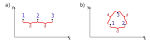
\includegraphics[width=0.9\textwidth]{./theory/physics/numerical-solutions/simple_case.pdf}}
    \vspace{-1.5cm}
    \caption{A representation of two simple latices. The spins are fixed at the point of the numbered locations. All sites have the same distance $d$ from each other. Note, that a spin up \up is directed parallel to the z-axis. That means in this case it would point out of the paper in the direction of the viewer.}
    \label{fig:simpleThreeLatticeIsing}
\end{figure}

In the beginning one trivial example will be discussed. The lattice is visualized in \autoref{fig:simpleThreeLatticeIsing}, image a).
This corresponds to a linear lattice in 1D. Let the Hamiltonian be the one in \ref{eq:hamiltonianExampleA}.

\begin{equation}
    \label{eq:hamiltonianExampleA}
    \hamiltonian = \sigma^z_1\sigma^z_2 + \sigma^z_2\sigma^z_3
\end{equation}

This hamiltonian is anti-ferromagnetic ($J = +1$). It should be easily seen, that the Energy $E$ in \ref{eq:schroedinger-general} becomes minimal (largest magnitude with negative sign) when the spins always point into the opposite direction as their neighbors: $\ket{\up, \down, \up}$ or $\ket{\down, \up, \down}$. This is quite a crucial step, so trying this by one self is advised for someone without prior quantum mechanical experience.
The ground state therefore will be a \emph{superposition} consisting of equal parts $\ket{\up, \down, \up}$ and $\ket{\down, \up, \down}$ \ref{eq:solutionSimpleExample}. The factor $\frac{1}{\sqrt[]{2}}$ instead of the seemingly more obvious $\frac{1}{2}$ makes the wavefunction be \emph{normalized}. If it wasn't for the square root, \autoref{eq:base-orthonormal} would not be satisfied. This way it is satisfied, which can be tested.

\begin{equation}
    \label{eq:solutionSimpleExample}
    \Psi_\mathrm{gnd} = \frac{1}{\sqrt[]{2}} \cdot \ket{\up, \down, \up} +  \frac{1}{\sqrt[]{2}} \cdot \ket{\down, \up, \down}
\end{equation}

The second example, visualized in \autoref{fig:simpleThreeLatticeIsing}, image b), however is not so simple. The corresponding hamiltonian can be seen in \ref{eq:hamiltonianExampleB}.
\begin{equation}
    \label{eq:hamiltonianExampleB}
    \hamiltonian = \sigma^z_1\sigma^z_2 +\sigma^z_2\sigma^z_3 +\sigma^z_1\sigma^z_3
\end{equation}
It has one more interaction than the previous one. Even though it also is anti-symmetric, it is \emph{not} possible to align all three spins in a way, so that they stand anti-parallel to all their neighbors. This phenomenon is called \emph{frustration} \cite*{frustration}.

Already this minimal problem has a complex superposition of eight base states as a ground state. The introduction of the transverse field will only make this more complex. Therefore a systematic way of finding the solution will be presented.

For this purpose, the example from \autoref{fig:simpleThreeLatticeIsing}, image b) will be used once more, but this time with the hamiltonian \ref{eq:hamiltonianExampleTransverse}.
\begin{equation}
    \label{eq:hamiltonianExampleTransverse}
    \hamiltonian = J\cdot \sigma^z_1\sigma^z_2 +J\cdot\sigma^z_2\sigma^z_3 +J\cdot\sigma^z_1\sigma^z_3
    +h \sigma^x_1+h \sigma^x_2+h \sigma^x_3
\end{equation}

The goal is now, to write the hamiltonian \hamiltonian as a matrix. 
The elements of the matrix should be $\bra{m}\hamiltonian\ket{n}$. Where $\ket{m}$ and $\ket{n}$ are two states out of the chosen basis. In this case the eight base states are the following:

\begin{center}
    \begin{tabular}{llll} 
        1: $\ket{\up, \up, \up}$ & 2: $\ket{\up, \up, \down}$  & 3: $\ket{\up, \down, \up}$  & 4: $\ket{\up, \down, \down}$ \\
        5: $\ket{\down, \up, \up}$ & 6: $\ket{\down, \up, \down}$  & 7: $\ket{\down, \down, \up}$  & 8: $\ket{\down, \down, \down}$ 
    \end{tabular}
\end{center}

In \ref{eq:matrixElement} an example calculation of $\bra{2}\hamiltonian\ket{4}$ is presented.

\begin{equation}
    \label{eq:matrixElement}
    \begin{split}
        &\bra{\up, \up, \down} \hamiltonian \ket{\up, \down, \down} = \\\\ % new line
         \bra{\up, \up, \down} J\cdot \sigma^z_1\sigma^z_2 \ket{\up, \down, \down} +
         &\bra{\up, \up, \down} J\cdot \sigma^z_2\sigma^z_3 \ket{\up, \down, \down} +
         \bra{\up, \up, \down} J\cdot \sigma^z_1\sigma^z_3 \ket{\up, \down, \down} +\\
         \bra{\up, \up, \down} h\cdot \sigma^x_1 \ket{\up, \down, \down} +
         &\bra{\up, \up, \down} h\cdot \sigma^x_2 \ket{\up, \down, \down} +
         \bra{\up, \up, \down} h\cdot \sigma^x_3 \ket{\up, \down, \down}\stackrel{\ref{eq:pauli-transformation}, \ref{eq:pauli-many-body}}{=}\\\\ % new line
          \bra{\up, \up, \down} J\cdot  1 \cdot (-1) \ket{\up, \down, \down} +
         & \bra{\up, \up, \down} J\cdot (-1) \cdot (-1) \ket{\up, \down, \down} +
          \bra{\up, \up, \down} J\cdot  1 \cdot (-1) \ket{\up, \down, \down} +\\
          \bra{\up, \up, \down} h\cdot  1 \cdot \ket{\down, \down, \down} +
         & \bra{\up, \up, \down} h\cdot 1 \cdot \ket{\up, \up, \down} +
          \bra{\up, \up, \down} h\cdot  1 \cdot \ket{\up, \down, \up} =\\\\ % new line
          (-J)\cdot      \bra{\up, \up, \down}  \ket{\up, \down, \down} +
         & J\cdot        \bra{\up, \up, \down} \ket{\up, \down, \down} +
          (-J)\cdot      \bra{\up, \up, \down}  \ket{\up, \down, \down} +\\
          h\cdot         \bra{\up, \up, \down}  \ket{\down, \down, \down} +
         & h\cdot        \bra{\up, \up, \down} \ket{\up, \up, \down} +
          h\cdot         \bra{\up, \up, \down}  \ket{\up, \down, \up}\stackrel{\ref{eq:base-orthonormal}}{=}\\\\ % new line
          (-J)\cdot 0 + J\cdot 0 &+  (-J)\cdot 0 + h\cdot 0  + h\cdot 1 + h\cdot 0   = h 
    \end{split}
\end{equation}
        \FloatBarrier
        \subsection{Solutions with Neural Quantum States}
        \label{sec:theory-neuralquantumstates}
        As a direct numerical approach is not sufficient, more advanced methods needed to be developed. 
\emph{Iterative} approaches have shown to be quite effective. 
In these kind of methods, the goal is not to compute a full solution directly, but to start with a random solution and perform iterative updates to it. 
If a good update strategy is chosen, the solution may converge towards the desired solution.

Because of the iterative nature, it is not necessary to do a complete computation at once. 
As learned in \fullref{sec:theory-numericalsolution}, the memory requirement for storing a complete hamiltonian matrix representation is also exponential.
So even with unlimited time, a numerical calculation could be impossible because of limited available memory. 
The iterative methods get around this, by being able to chose a data structure with much higher information density than the full hamiltonian (For example if only the ground state is wanted, it is unnecessary to store anything but information regarding it. The hamiltonian though encodes a lot of \glqq unnecessary\grqq{} information about other states). This structure can then be iteratively refined.

In practice a so called \emph{neural quantum state} (NQS) is used. 
This basically is nothing but a neural network, taken from established machine learning tasks.
The function is parametrized by $M$ variables $\theta_i \in \mathbb{R}, 0\leq i < M$ and takes a spin configuration as an input.
A spin configuration for $N$ lattice sites can be described by $\sigma_j \in \left\{\up, \down\right\}, 0\leq j < N$.
The function will be written like \autoref{eq:parametrized-wavefunction}.

\begin{equation}
    \label{eq:parametrized-wavefunction}
    \ket{\Psi_{\theta_0, ..., \theta_{M-1}}(\sigma_0, ..., \sigma_{N-1})} \equiv \ket{\Psi_\theta}
\end{equation}

In order to compute a helpful representation, the identities \autoref{eq:completeness-of-base} and \autoref{eq:wave-function-probability} are necessary \cite{schwablQM}. \autoref{eq:completeness-of-base} applies to \emph{complete orthonormal} bases only.

\begin{equation}
    \label{eq:completeness-of-base}
    \sum\limits_{s} \ket{s}\bra{s} = \mathbb{1}
\end{equation}

\begin{equation}
    \label{eq:wave-function-probability}
    \bra{\Psi}\ket{\Psi} = \Psi^\ast\cdot \Psi = \left|\Psi\right|^2 \in \mathbb{R}
\end{equation}

The following method is described in \cite{jVMCPaper}.

To calculate the \emph{expectation value} of a quantum mechanical operator \operator for the wavefunction $\ket{\Psi}$, the expression 
$\frac{\bra{\Psi}\operator\ket{\Psi}}{\bra{\Psi}\ket{\Psi}}$ is used \cite{schwablQM}. The denominator assures, that the calculation is correct for \emph{non-normalized} wavefunctions (as the NQS is initialized randomly it very likely isn't normalized). 

Applying this to the problem at hand, the target is to measure the observable corresponding to \operator in the parametrized neural quantum state $\ket{\Psi_\theta}$.

\begin{equation}
    \label{eq:derivation-local-estimator}
    \begin{split}
        \frac{\bra{\Psi_\theta}\operator\ket{\Psi_\theta}}{\bra{\Psi_\theta}\ket{\Psi_\theta}} &\stackrel{\ref{eq:completeness-of-base}}{=}
        %
        \frac{\bra{\Psi_\theta} \left(\sum\limits_{s} \ket{s}\bra{s}\right)
        \operator \left(\sum\limits_{s'} \ket{s'}\bra{s'}\right) \ket{\Psi_\theta}}{\bra{\Psi_\theta}\left(\sum\limits_{s} \ket{s}\bra{s}\right)\ket{\Psi_\theta}}\\
        %
        &\stackrel{\phantom{\ref{eq:completeness-of-base}}}{=}
        \frac{\sum\limits_{s, s'} \bra{\Psi_\theta} \ket{s}\bra{s}
        \operator \ket{s'}\bra{s'} \ket{\Psi_\theta}}{\sum\limits_{s}\bra{\Psi_\theta}\ket{s}\bra{s}\ket{\Psi_\theta}}
        %
        \stackrel{\phantom{\ref{eq:completeness-of-base}}}{=}
        \frac{\sum\limits_{s} \bra{\Psi_\theta} \ket{s} \frac{\bra{s} \ket{\Psi_\theta}}{\bra{s} \ket{\Psi_\theta}} \sum\limits_{s'} \bra{s}
        \operator \ket{s'}\bra{s'} \ket{\Psi_\theta}}{\sum\limits_{s}\bra{\Psi_\theta}\ket{s}\bra{s}\ket{\Psi_\theta}}\\
        %
        &\stackrel{\phantom{\ref{eq:completeness-of-base}}}{=}
        \sum\limits_{s} \frac{ \bra{\Psi_\theta} \ket{s}\bra{s} \ket{\Psi_\theta} \sum\limits_{s'} \bra{s}
        \operator \ket{s'} \frac{\bra{s'} \ket{\Psi_\theta}}{\bra{s} \ket{\Psi_\theta}}}{\bra{\Psi_\theta}\ket{s}\bra{s}\ket{\Psi_\theta}}
        %
        \stackrel{\ref{eq:local-estimator}}{=}
        \sum\limits_{s} \frac{ \bra{\Psi_\theta} \ket{s}\bra{s} \ket{\Psi_\theta} \operator_\mathrm{loc}^\theta(s)}{\bra{\Psi_\theta}\ket{s}\bra{s}\ket{\Psi_\theta}}\\
        %
        &\stackrel{\ref{eq:base-factors}}{=}
        \sum\limits_{s} \frac{ \Psi_\theta(s)^\ast \cdot \Psi_\theta(s) \cdot \operator_\mathrm{loc}^\theta(s)}{\Psi_\theta(s)^\ast \cdot \Psi_\theta(s)}
        %
        \stackrel{\ref{eq:wave-function-probability}}{=}
        \sum\limits_{s} \frac{ \left|\Psi_\theta(s)\right|^2  \operator_\mathrm{loc}^\theta(s)}{\left|\Psi_\theta(s)\right|^2}
    \end{split}
\end{equation}

In the derivation, the \emph{local estimator} (\autoref{eq:local-estimator}) is introduced. Because the computational base is sparse, only very few elements of the sum over $s'$ in \autoref{eq:local-estimator} are non-zero \cite{jVMCPaper}. A local estimator can therefore be evaluated in constant time.

\begin{equation}
    \label{eq:local-estimator}
    \operator_\mathrm{loc}^\theta(s) = \sum\limits_{s'} \bra{s} \operator \ket{s'} \frac{\bra{s'} \ket{\Psi_\theta}}{\bra{s} \ket{\Psi_\theta}}
\end{equation}

The final result in \autoref{eq:derivation-local-estimator} has the form of a \emph{probability distribution} over $s$.
So the calculation of a expectation value can be re-formulated as the calculation of the expectation value of $s$ of the local estimator (which can be evaluated in constant time).

This alone is not helpful, because $\ket{s}$ is still exponentially large in regards to the problem size.
But this shortcoming can be resolved with the introduction of \emph{Monte Carlo} sampling.
The \emph{probability density} can be estimated, by looking at only a subset of possible $\ket{s}$.

By randomly sampling a large, but manageable number $N_\mathrm{MC}$ of states $s_{(n)}$ with the \emph{Metropolis algorithm} \cite{quantumMonteCarloSimulationsOfSolids}, the true value can be approximated (\autoref{eq:mc-local-estimator}) \cite{jVMCPaper}.

\begin{equation}
    \label{eq:mc-local-estimator}
    \frac{\bra{\Psi_\theta}\operator\ket{\Psi_\theta}}{\bra{\Psi_\theta}\ket{\Psi_\theta}} \approx
    \frac{1}{N_\mathrm{MC}} \sum\limits_{n=1}^{N_\mathrm{MC}} \operator_\mathrm{loc}^\theta(s_{(n)})
\end{equation}

Therefore the energy of a system can be estimated with \autoref{eq:energy-optimization}. All the terms can efficiently be computed, using methods from \fullref{sec:theory-numericalsolution}.

\begin{equation}
    \label{eq:energy-optimization}
    E(\theta) = \frac{\bra{\Psi_\theta}\hamiltonian\ket{\Psi_\theta}}{\bra{\Psi_\theta}\ket{\Psi_\theta}} \approx
    \frac{1}{N_\mathrm{MC}} \sum\limits_{n=1}^{N_\mathrm{MC}} \hamiltonian_\mathrm{loc}^\theta(s_{(n)}) \stackrel{\ref{eq:local-estimator}}{=}
    \frac{1}{N_\mathrm{MC}} \sum\limits_{n=1}^{N_\mathrm{MC}} \left(\sum\limits_{s'} \bra{s_{(n)}} \hamiltonian \ket{s'} \frac{\bra{s'} \ket{\Psi_\theta}}{\bra{s_{(n)}} \ket{\Psi_\theta}}\right)
\end{equation}

As it is known, that the ground state energy $E_0$ is the smallest energy, the ground state can be estimated in the following way:
\begin{enumerate}
    \setlength\itemsep{-0.5em}
    \item Start with a randomly initialized NQS
    \item Estimate its energy with \autoref{eq:energy-optimization} and MC-sampled states
    \item Calculate the neural network error, assuming $E(\theta)$ should be smaller (formula in \cite{jVMCPaper})
    \item Propagate the error back into the network
    \item Repeat at 2. with the updated NQS
\end{enumerate}

Because the method iteratively updates the network by performing tiny variations, it is called \emph{variational Monte Carlo} (VMC) method.

        \FloatBarrier
        \subsection{Imaginary Time Evolution}
        \label{sec:theory-imagenarytimeevolution}
        Many different iterative methods are being employed to calculate the desired physical quantities.
In this section, a mathematical idea will be discussed, that has several applications.
The method is employed in the \emph{diffusion Monte Carlo} method (DMC) \cite{quantumMonteCarloSimulationsOfSolids}, a second application of Monte Carlo sampling in comparison to VMC.

This section is about more advanced quantum mechanical principles and requires prior experiences. It is of supplemental nature and can therefore be skipped without sacrificing on the possibility to understand subsequent parts of the thesis.

The method is described in \cite{imaginarySchroedingerEquation}.

\autoref{eq:schroedinger-general} can be generalized to be no longer time independent. 
\autoref{eq:schroedinger-td} is called the \emph{time-dependent Schrödinger equation}. $\hbar$ is the \emph{reduced Planck constant}, $t$ is the time.

\begin{equation}
    \label{eq:schroedinger-td}
    \hamiltonian \ket{\Psi(t)} = i\hbar \frac{\partial }{\partial t} \ket{\Psi(t)}
\end{equation}

In this case, the wavefunction also needs to depend on the time as a variable.
For a time-independent hamiltonian, the time dependent wavefunction can be obtained via \autoref{eq:timeEvolutionWavefunction} \cite{schwablQM} with the energy eigenvalues $E_n$ ($E_0$ being the ground state energy), the energy eigenbase states $\ket{n}$ and the wavefunction at time $t=0$, $\ket{\Psi(0)}$.

\begin{equation}
    \label{eq:timeEvolutionWavefunction}
        \ket{\Psi(t)} = e^{-i\hamiltonian t / \hbar} \ket{\Psi(0)}
\end{equation}

That \autoref{eq:timeEvolutionWavefunction} is a solution to \autoref{eq:schroedinger-td} can be verified like in \autoref{eq:validationTimeEvolution} (notice that the hamiltonian is time-independent).

\begin{equation}
    \label{eq:validationTimeEvolution}
    \begin{split}
        i\hbar \frac{\partial }{\partial t} \ket{\Psi(t)} &\stackrel{\ref{eq:timeEvolutionWavefunction}}{=} 
        i\hbar \frac{\partial }{\partial t}  e^{-i\hamiltonian t / \hbar} \ket{\Psi(0)}\\
        &\stackrel{\phantom{\ref{eq:timeEvolutionWavefunction}}}{=} \frac{-i\cdot i \hamiltonian \hbar}{\hbar} e^{-i\hamiltonian t / \hbar} \ket{\Psi(0)}\\
        &\stackrel{\ref{eq:timeEvolutionWavefunction}}{=} \hamiltonian \ket{\Psi(t)}
    \end{split}
\end{equation}

\autoref{eq:timeEvolutionWavefunction} can be rewritten in terms of the energy eigenbase.

\begin{equation}
    \label{eq:rewriteTimeEvolutionWavefuntion}
    \begin{split}
        \ket{\Psi(t)} &\stackrel{\phantom{\ref{eq:base-change}, \ref{eq:base-factors}}}{=} e^{-i\hamiltonian t / \hbar} \ket{\Psi(0)} \\
        &\stackrel{\ref{eq:base-change}, \ref{eq:base-factors}}{=}
        \sum\limits_{n}^{} e^{-i \hamiltonian t / \hbar} \bra{n}\ket{\Psi(0)} \ket{n}\\
        &\stackrel{\phantom{\ref{eq:base-change}, \ref{eq:base-factors}}}{=}
        \sum\limits_{n}^{} e^{-i E_n t / \hbar} \bra{n}\ket{\Psi(0)} \ket{n}
    \end{split}
\end{equation}

In \autoref{eq:rewriteTimeEvolutionWavefuntion}, an operator gets applied from inside an exponent. This can be explained with the possibility to express the $e$-function in terms of its \emph{Taylor series} \cite{schwablQM}. This is important to understand the transition from \hamiltonian to $E_n$ in the exponent. For the transformation, the function is written as its Taylor series, the operator gets applied and then the Taylor series is reversed into the function. Remember that $\bra{n}\ket{\Psi(0)}$ is simply a complex number.

The method is called \emph{imaginary} time evolution, because of the step in \autoref{eq:complexTimeVariableChange}.

\begin{equation}
    \label{eq:complexTimeVariableChange}
    \tau = i\cdot t
\end{equation}

An \glqq imaginary\grqq{} time $\tau$ can be obtained by equation \autoref{eq:complexTimeVariableChange}. Switching variables in \autoref{eq:rewriteTimeEvolutionWavefuntion} leads to the representation shown in \autoref{eq:complexTimeExponential}.

\begin{equation}
    \label{eq:complexTimeExponential}
    \ket{\Psi(\tau)} = \sum\limits_{n}^{} e^{-E_n \tau / \hbar} \bra{n}\ket{\Psi(0)} \ket{n}
\end{equation}

$E_0 > 0$ can be assumed without loss of generality.
It is known by definition, that $E_0 \leq E_j, j\neq 0$. 
\autoref{eq:complexTimeExponential} contains only terms, that decay exponentially with $\tau$.
Because of that, for large values of $\tau$ all terms decay to 0, but the $n=0$ term decays the slowest. \autoref{eq:complexTimeApplication} is therefore won.

\begin{equation}
    \label{eq:complexTimeApplication}
    \lim\limits_{\tau \rightarrow \infty}\frac{\ket{\Psi(\tau)}}{e^{-E_0 \tau / \hbar}} \stackrel{\ref{eq:complexTimeExponential}}{=} \bra{0}\ket{\Psi(0)} \ket{0}
\end{equation}

This means, that if the starting wavefunction has an overlap with the ground energy eigenstate ($\bra{0}\ket{\Psi(0)} \neq 0$), if the wavefunction is evolved in imaginary time, all contributions except the ground state contribution will be eliminated.

This can be used to find the ground state \cite{quantumMonteCarloSimulationsOfSolids}. A random starting function is chosen and evolved in complex time with the aid of Monte Carlo sampling. The ground state can then be extracted. If there is no overlap between the starting function and the ground state, the method converges to the base state with the smallest energy that also has overlap.
        \FloatBarrier
        \subsection{Explored Lattice Patterns}
        \label{sec:theory-latticepatterns}
        In \autoref{fig:simpleThreeLatticeIsing} two examples of lattice-shapes were already introduced.
In the research leading to this thesis, a selection of lattices were chosen.
The implementation supports a 1D lattice (the default \textbf{linear} lattice/chain  (\autoref{fig:appendix-linear-lattices})) and five different 2D lattices 
(\textbf{cubic} (\autoref{fig:appendix-cubic-lattices}), \textbf{hexagonal} (\autoref{fig:appendix-hexagonal-lattices}), \textbf{trigonal\_square} (\autoref{fig:appendix-trigonal_square-lattices}), \textbf{trigonal\_hexagonal} (\autoref{fig:appendix-trigonal_hexagonal-lattices}) and \textbf{trigonal\_diamond} (\autoref{fig:appendix-trigonal_diamond-lattices})).

The lattice structure can be interactively visualized with the use of \cite{selfDocuments} \filepath{/structures/visualize.py}.
The same code was used to generate the referenced visualization printed in the \nameref{sec:appendix}.

The numbers, that can be seen in the visualization denote the location-index of the memory, that is responsible for carrying the spin state at that lattice site in the later representation. As will become obvious in \fullref{sec:theory-graphs}, the structure of a lattice cannot always be represented directly analogous in memory. Therefore an alternative way of addressing lattice sites and theirs surroundings needs to be employed.
In this case, the framework generates the set of \emph{nearest neighbor} (marked green in the visualization) and \emph{next-nearest neighbor} (marked yellow in the visualization) indices for a given lattice site (marked red in the visualization). These are used as structural inputs for later discussed \emph{graph} architectures.

A quite important feature for the physical aspect of the calculation is the \emph{periodicity} of a lattice. 
As real world crystals have many magnitudes more lattice sites than can be simulated currently, \emph{boundary effects} play a significant role in simulated latices.
This often times is an unwanted manner, if the goal is to calculate the behavior of the system far away from the edges. 
Lattices should there have the property of \emph{translational symmetry}. 
To aid with this, a \emph{periodic} repetition of the lattice can be toggled. 
It is responsible for defining neighbors for lattice sites close to the edges of the lattice.
The \nameref{appendix:lattice-visualisation} in the appendix shows this, by providing the information whether the pictured lattice is periodic or not.

The way in that the lattices are tiled is should become clear from the visualization.
It is noteworthy, that the \textbf{cubic}, \textbf{trigonal\_square} and \textbf{trigonal\_diamond} lattices have repetition along two axes, while the \textbf{hexagonal} and \textbf{trigonal\_hexagonal} have three. 
The hope is that the \textbf{trigonal\_hexagonal} and \textbf{trigonal\_square}/\textbf{trigonal\_diamond} lattices show the same behavior in non-periodic mode (as they all three represent a trigonal lattice), while differences manifest in periodic inspection.

Last, there is a setting to \emph{randomly swap} lattice positions. 
The effect of this can be seen in \autoref{fig:direct-comparison-lattice-site-swaps}.

\begin{figure}[htbp]
    \centering
    \makebox[\textwidth][c]{
        \includegraphics[width=0.3\textwidth]{./theory/physics/explored-lattice-patterns/hexagonal,size=2,np.pdf}
        \includegraphics[width=0.3\textwidth]{./theory/physics/explored-lattice-patterns/hexagonal,size=2,np,rs=2.pdf}
    }
    \makebox[\textwidth][c]{
        \includegraphics[width=0.3\textwidth]{./theory/physics/explored-lattice-patterns/trigonal_square,size=3,np.pdf}
        \includegraphics[width=0.3\textwidth]{./theory/physics/explored-lattice-patterns/trigonal_square,size=3,np,rs=-1.pdf}
    }

    \vspace{0.2cm}
    \caption{Visualization of the property \emph{random swaps} of the lattice structure helper. In the first set of figures, two swaps were performed on a hexagonal lattice of size 2 (8 with 15 and 16 with 21). The neighbor-index calculation takes this into effect, therefore the highlighted lattice sites do not change. The second set of figures shows the setting -1 for a trigonal\_square lattice of size 3. This basically makes the generator perform such a high number of pair swaps, so that the index-position correlation can be taken as randomly. 
    }
    \label{fig:direct-comparison-lattice-site-swaps}
\end{figure}

The goal of this setting is to decouple the in-memory representation and the structure of the simulated lattice. 
Effects of this will be explored in \fullref{sec:experiments-resiliencylatticeencoding}.
        \FloatBarrier
    \section{From the Point of Computer Science}
        \label{sec:theory-cs}
        % TODO

% SOURCE: \cite{pytorchGithub}
% SOURCE: \cite{dinoGithub}
% SOURCE: \cite{einopsGithub}
% SOURCE: \cite{positionalEncodingGithub}
% SOURCE: \cite{poolformerGithub}

        \FloatBarrier
        \subsection{The Image Classification Task}
        \label{sec:theory-imageclassification}
        It has been more than 30 years, since it was proven, that already simple neural network architectures can in fact be \emph{universal approximators} \cite*{ffnUnversalApproximator}. 
That means that if a problem can be formulated as a mathematical function, this function can be approximated by a neural network.
This has huge consequences, because if input and output are encoded digitally in a predefined format, \emph{all} mappings between these can be formulated in form of a mathematical function. 
Be it only the trivial one, that maps each input encoding to the desired output encoding.
Because of that, seemingly impossibly complex problems can be tackled now days. 

Part of the experimentation in the thesis will focus on the application of a select breed of neural networks on the \emph{image classification task}.
This is not a novel problem, but one that has been triad and soled by many teams of researchers. 
The gist is, to build a neural network that can label the things pictured on some kind of image.
In our case, an even simpler version of the problem will be considered. 
The only job of the network is, to select one of $N$ predefined labels, that describe the picture best.

The architecture of the network can be viewed generalized in \autoref{fig:immage-classification-general}.

\begin{figure}[htbp]
    \centering
    \makebox[\textwidth][c]{\includegraphics[width=\textwidth]{./theory/cs/image-classification/process.pdf}}
    \caption{Generalized schema of the image classification pipeline used in the experiments portion of this thesis.
        The image gets rasterized, resized to 224$\times$224 pixel and 8 bit color depth. Then the image is normalized, reshaped into vector form and processed from there. The MLP in this image is only a placeholder. Many of the later discussed neural network architectures treat the reshaping, casting and processing differently. The output for all networks needs to be in form of 100 floating point numbers. the one closest to one gets selected as the networks choice. The class name, the index represents can then be looked up.
        Cat image from \cite{catPhoto}.
    }
    \label{fig:immage-classification-general}
\end{figure}

        \FloatBarrier
        \subsection{Neural Network Training}
        \label{sec:theory-neuralnetworktraining}
        When initializing neural networks, they most often come only with an empty structure, that allows for the possibility to acquire a computing machine if all the internal parameters and weights are set accordingly.
For very small computational networks, it is possible to set the weights by hand.
But already for low tens or hundreds of numbers this becomes an unfeasible task. 

Because of that, neural networks are \emph{trained} to get them into a working state. In the training phase the structure of the network is (normally) left static, only the parameter values are adjusted. 
The algorithm that accomplishes an update of the weights, that nudges the network \emph{towards} the desired solution, is called \emph{backpropagation} \cite{machineLearningMitchell}.
It is based on the chain rule of differentiation and uses the severity of changes a parameter inflicted on a (intermediate) result, to update the parameter in a way, that steers said result towards the desired one. 

As mentioned, for one run, the structure is typically unchanged. 
The general shape of the network and many turning knobs on the update process can be controlled to allow for a more efficient representation and weight update.
The controlling variables are called \emph{hyperparameters}.
The most important hyperparameters in the later experiments will be the \emph{optimizer} (\emph{stochastic gradient descent} and \emph{adamw} \cite{adamwOptimizer} are compared), the \emph{loss function} (\emph{cross entropy loss} is used), and the \emph{batch size}. 
Additionally, the \emph{learning rate}, \emph{weight decay}, \emph{dampening} and \emph{momentum} can be set to modify the behavior of the optimizer.

Different optimizers change the updating behavior of the network. 
The loss function defines a measure on how far or close the computed solution is in comparison the the known solution.
The learning rate defines the step size that gets taken towards the target in one iteration.
Choosing its value too small results in slow convergence, choosing a value too big can result in overshooting and subsequently also lowering the speed of convergence.
Dampening and momentum are generally used to combat either of these effects.
Weight decay generally helps against \emph{overfitting} (If a model's generalization capacity is exhausted or the training examples are to monotone, this can lead to memorization of a subset of training examples. This increases the performance on training data, but hurts the performance on unseen data). 
As for our applications, overfitting is unimportant or even desired (see \autoref{sec:biases}), this parameter left unchanged.

The article \emph{A ConvNet for the 2020s} \cite{convNetForThe2020s} makes the point, that by heavily investing in choosing the appropriate hyperparameters, state of the art performance can be extracted even from \glqq standard\grqq{} model architectures. 
As the focus in this thesis is to compare the performance of different \emph{architectures} with each other, \emph{no efforts} are made to tune hyperparameters to achieve the absolute best performance. 
In contrary, hyperparameters were left \emph{deliberately} static, to allow for a more fair comparison where possible.

One more important parameter is the batch size. 
By processing more than one training example at a time, a more stable and efficient update process can be achieved.
However the batch size is limited by the available memory. 
As most of the calculations are performed on a GPU, the video memory is important. 
The calculations were either performed on a \emph{NVIDIA GeForce GTX 1070} with \SI[]{8}[]{GB} of video memory or a \emph{NVIDIA TITAN Xp} with \SI[]{12}[]{GB}. 
Both cards are mid to low range in performance and video memory, in comparison to the most up to date cards. 
Therefore often the batch size and number of iterations had to be set lower than may be desirable for an optimal result. Though it speaks in favor of the applied methods, that good results could be achieved without top-tier hardware.

Very important for generating training data for an image recognition task are the \emph{augmentations}. 
They are a big focus of the research performed in \cite{convNetForThe2020s} and \cite{dinoPaper}.
As transformer models generally require really large datasets to train, it is desirable to generate more data from the data that is already collected. 
This can be achieved by augmenting the training images in a way that does not change the content according to human recognition, but produces a different input for the network.
Flipping, rotating, cropping or adding noise to an image are all possible augmentations. 
In the experiments only random horizontal flips are employed, to (hopefully) still be able to overfit all models. 
This is necessary to be able to judge the models \emph{inductive bias} (\autoref{sec:biases}).

To paint a more complete picture, there are other strategies, than just forcefully training a model directly from scratch. 
Some of those will be be presented in the following section.
        \FloatBarrier
        \subsection{Neural Network Pre-Training}
        \label{sec:theory-pretraining}
        As a human it is often complicated to jump into an unfamiliar task and learn everything necessary to solve it at once.
The same is true for neural networks. 
Different strategies have been devised to combat this difficulty. 
None of them is applied in the experiments section of this thesis. 
However it may be fruitful to look into their application in further research. 

One method is to \emph{distill} knowledge from one network to the other. 
For that strategy, first a large and expensive network could be trained.
Then a smaller network is trained with the task to replicate the behavior of the complex network. 
This method among other things is discussed as a complementary measure in \cite{mobileNetPaper}.
The idea is, that by forcing the information into less weights, a higher level of abstraction and problem extrapolation can be achieved, and pure memorization of the solutions is less likely.

An \glqq online\grqq{} approach to this method are \emph{teacher-pupil} methods. 
By training multiple networks in parallel and motivating them to outperform each other, a better performance can be achieved. This is an important point in \cite{dinoPaper}.

Finally, very large performance gains can be won from the employment of \emph{pre-training}.
This method resembles the human learning strategy to first acquiring general knowledge about a problem by segmenting it into basic blocks and practicing on them.
Then learning to refine the general knowledge into one that solves a specific task.

Pre-training in \emph{language processing} is a key aspect of the research in \cite{bertPaper}.
A neural network could for example be trained to reconstruct a sentence, of which one word has been masked out.
Generating labeled training data for such cases is basically trivial. 
Therefore the neural network can learn a lot about word proximity and basic sentence structures.
Because it is a highly labor intensive process to acquire texts with verified and suited translations alongside them, a network with pre-trained knowledge of sentence structure and linguistic mannerisms can extract knowledge from this limited data more efficiently and quickly.
The process of adapting a pre-trained network to a desired task is called \emph{fine-tuning}.

The datasets in pre-training are generally larger and easier to generate. 
For example for images, letting a network \emph{cluster} a vast amount of images into a predefined number of categories will force it to extract information about similarities and regularities among the pictures, while not requiring the image to be labeled. This approach therefore is called an \emph{unsupervised} pre-training \cite{dinoPaper}. 
The clustering may not group the images into the same categories as a human wants the network to group them, but it is very likely that important features must be taken into account somehow. 
A smaller, labeled training set can then be used to fine-tune the networks prediction to reflect the desired output mapping. 
Pre-training is integral to the use of transformers for image recognition \cite{imageWorth16x16}. 

However as this thesis focuses on the performance of different types of architectures and not on the extraction of maximum efficiency from one network, no pre-training is used in the following experiments.

        \FloatBarrier
        \subsection{Employment of Graphs for Problem transfer}
        \label{sec:theory-graphs}
        When using data for training neural networks, a consistent \emph{encoding} has to be used.
In \autoref{fig:image-classification-general} an image is transformed into a neural network input by reshaping its pixels into one column of numbers. This also works for images with multiple color channels.
A highly useful property of images is, that they can directly be encoded into \emph{tensors} depending on their format (e.g. a $224\times224$ matrix for a grayscale image or a $3\times224\times224$ tensor for an image with three color channels).

By leaving this structure in the way it already is stored in, properties like the pixel-proximity relation is conserved (while reordering into one column obviously does not preserve this information in the same way).
Network elements like \emph{convolutions} (\autoref{sec:architectures-convolution}) can take advantage of this preserved information. 
The utilization of such kind of information is called an \emph{implicit bias} and discussed in detail in \autoref{sec:biases}.

The canonical representation of images in memory is also the reason, why GPUs (\emph{graphics} processing units) are highly optimized to run calculation on tensors.
Because of their hardware design, operations like matrix multiplication or tensor addition can be carried out highly parallelized and efficiently.
The hardware was originally designed to render graphics to the computer screen. 
It is however no longer used exclusively for that.
If a computational problem can be reduced to solving a matrix calculation, it can easily be carried out by a GPU.

But not all data is generally representable in tensor form. A common data structure - in that many nodes exist which have relations defined between them - is called a \emph{graph}.
Examples for graph data are social media friendship relations or street data inside a navigational system.
As graphs are quite versatile however, a lot of things can be represented with them.

The novel concept is, to represent the lattice structures from \autoref{sec:theory-latticepatterns} as a graph and then apply neural network architectures, that are specifically designed to deal with that kind of data.

A big advantage is, that as graphs are more versatile than the strict tensor representation, the tensor data of an image can \emph{also} be represented as a graph. 
A square picture can for example be represented as a graph, if every pixel is treated as its own node. 
By connecting the neighboring pixels with edges, the problem can be transferred into a graph representation, without losing the information about the proximity of pixels in relation to each other.

Established operations like \emph{pooling} (\autoref{sec:architectures-perceptron-pooling}) or \emph{convolutions} (\autoref{sec:architectures-convolution}) can be defined to work on graph data. 
That will be done in \autoref{sec:architectures-graphs}. 
The advantage of the possibility to represent images in both encodings is, that the functionality of the graph operators can be verified and compared against the established implementations for tensors.
That way, one can be confident, that the calculations will also work for data that is \emph{not} representable in a tensor form.

As a graph with one node per pixel of an image would be quite large - even for low resolution images - larger chunks of the image, called a \emph{patch} (e.g. $16 \times 16$ pixel) can be treated as one unit. 
With that method, localized interactions can be computed inside a patch, while mid to far range interactions can be computed between nodes/patches, while at the same time drastically cutting down the number of nodes in the graph.

Patching has already been used extensively in \emph{vision transformer} architectures (\autoref{sec:architectures-attention}) \cite{dinoPaper, imageWorth16x16}. 
The graph-versions of these transformers are however relatively uncommon.

% SOURCE: \cite{bertPaper}
% - importance of bi-directional nature, that can look into the future (for us important, as there is not time axis in images and everything can be seen at once)
% -> decided against using that source here, because talking about image and language processing over complicates the section
        \FloatBarrier

\chapter{Machine Learning Architectures}
\label{sec:architectures}

    \section{Used Architectures}
    \label{sec:architectures-theory}
    % TODO

% SOURCE: \cite{pytorchGithub}
% SOURCE: \cite{dinoGithub}
% SOURCE: \cite{einopsGithub}
% SOURCE: \cite{positionalEncodingGithub}
% SOURCE: \cite{poolformerGithub}

        \subsection{Perceptron and Pooling Architectures}
        \label{sec:architectures-perceptron-pooling}
        In the most basic sense, all neural network operators need to be able to take in a set of numbers and perform calculations on them, then provide an output.
The shape can change from input to output, depending on the operator.
Some operators, like the \emph{perceptron} (or its conceptual successors, the \emph{fcl} and \emph{MLP}) have trainable weights that get updated like described in \autoref{sec:theory-neuralnetworktraining}.
Others, like the \emph{pooling operator} transform the data according to static rules, without trainable parameters.
A neural network can't be trained, if it doesn't contain operators with adjustable weights.
However operators like pooling are very efficient in supporting trainable operators (as will be shown later).

\paragraph{The perceptron} is the most basic building block of all neural network architectures.
A schematic view is given in \autoref{fig:perceptron}.

\begin{figure}[htbp]
    \centering
    \makebox[\textwidth][c]{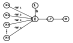
\includegraphics[width=0.6\textwidth]{./architectures/theory/perceptron-pooling/perceptron.pdf}}
    \caption{Schematic representation of a perceptron. Inputs are denoted with $x_i$, weights with $w_i$, the bias value with $b$ and the output with $o$. 
        The inputs get scaled with the weights, summed and the bias is added.
        Then the value is passed through a not specified non-linear function (e.g. ReLU or the sigmoid function).
    }
    \label{fig:perceptron}
\end{figure}

The output gets calculated like $o = \mathrm{ReLU} \left(\sum\limits_{i=1}^{n} x_i\cdot w_i + b\right)$.
Calculating multiple perceptrons with different weights in parallel for the same input values $x$ is called a fully connected layer (fcl).
The formula for the elements in a fcl is show in \autoref{eq:fcl},

\begin{equation}
    \label{eq:fcl} 
    o_j = \sum\limits_{i=1}^{n} x_i\cdot w_{i, j} + b_j
\end{equation}

which is equivalent to a matrix-vector-multiplication. Therefore the fcl can be evaluated quickly.
\autoref{fig:image-classification-general} shows multiple fcls in series, which is called a multi layer perceptron (MLP). 

\paragraph{The pooling operator} is basically a function that selects a new value based on values in a specific range around the target position.
The rules can range from taking the \emph{minimal} value, to the \emph{maximum} value or the \emph{average}.
In this thesis, all pooling operations are average pooling.

\begin{figure}[htbp]
    \centering
    \makebox[\textwidth][c]{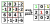
\includegraphics[width=0.6\textwidth]{./architectures/theory/perceptron-pooling/pooling.pdf}}
    \vspace{-0.2cm}
    \caption{
        Example for a 2$\times$2-average-pooling operation. The colors indicate what numbers get averaged. 
        Not all blocks are colored, but the calculation is performed analogously.
    }
    \label{fig:pooling}
\end{figure}

\autoref{fig:pooling} shows an example of an 2$\times$2-average-pooling operation.
Where the dimension of input and output need to stay the same, the border of the input is padded with zero values (no padding in this example).
        \FloatBarrier
        \subsection{Convolutional Architectures}
        \label{sec:architectures-convolution}
        The convolution operation is a combination of concepts from the fcl and pooling.
Like in pooling, values get aggregated from inside a specific region of influence.
They do however not get treated uniformly, but scaled with (learnable) weights before being summed up.

The comparison between a \emph{normal convolution}, a \emph{depthwise convolution} and a \emph{depthwise separable convolution} is given in \autoref{fig:comparison-depthwise-convolution}.

\begin{figure}[htbp]
    \centering
    \makebox[\textwidth][c]{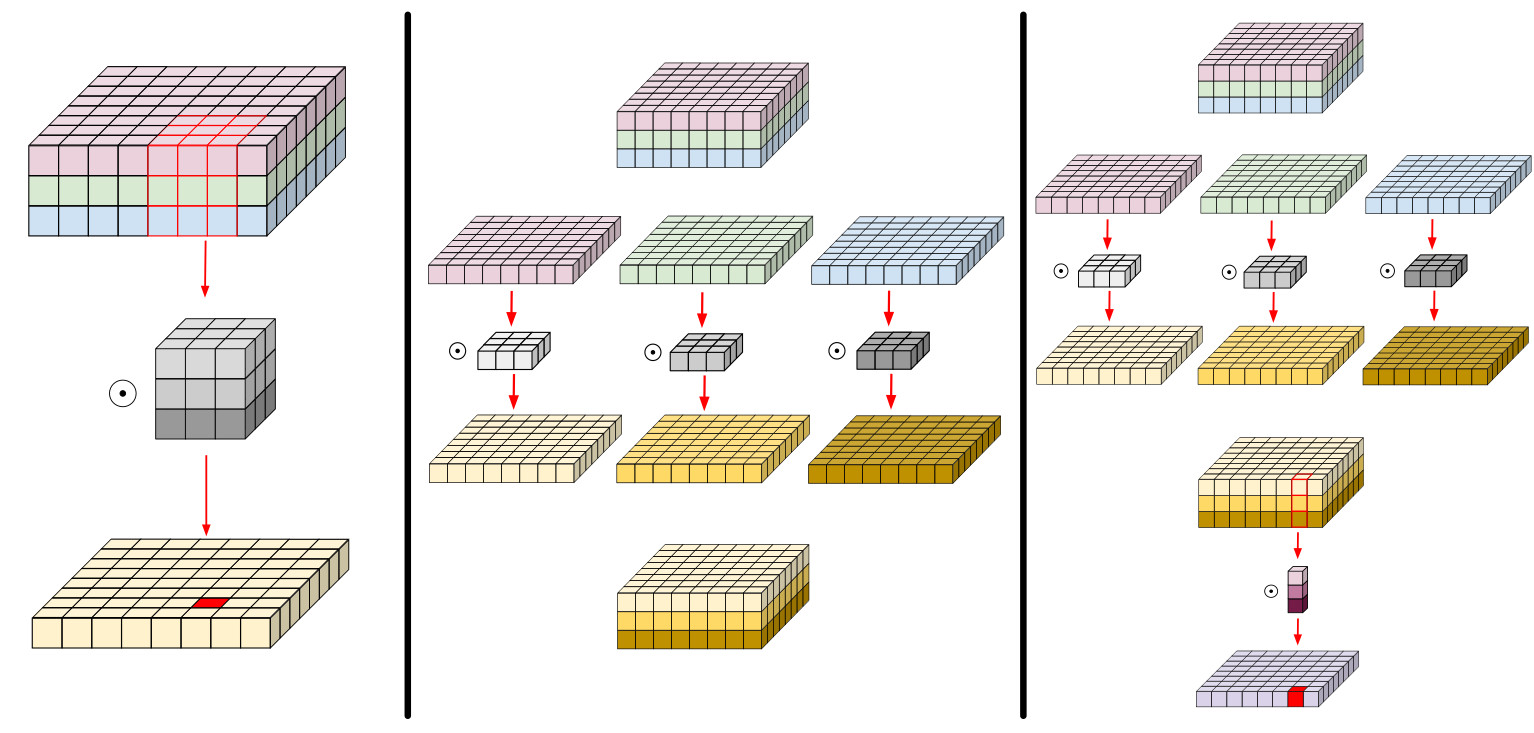
\includegraphics[width=1.1\textwidth]{./architectures/theory/convolutions/depthwise.pdf}}
    \caption{This figure show the differences between a \emph{normal convolution} (left), a \emph{depthwise convolution}  (middle) and a \emph{depthwise separable convolution} (right).
    The normal convolution has a 3D-kernel. The depthwise convolution splits this into multiple 2D-kernels.
    The depthwise separable convolution works basically in the same way as the depthwise, but at the end a 1D-kernel (1$\times$1-convolution) is used to combine the channels.
     Original image from \cite{separableConvolutions}, but modified and almost completely redrawn.}
    \label{fig:comparison-depthwise-convolution}
\end{figure}



The implementation of the symmetric depthwise convolution for images can be found at \cite{selfComputerScience}, \filepath{/models/helpers/SymmConv2d.py}.


% - focus on differences between depthwise and normal convolution
% - symmetrical convolutions with shared weights and their implementation 

% SOURCE: \cite{mobileNetPaper}
% - reduce network size and costs to be able to ship for low power/storage mobile devices

% SOURCE: \cite{channelNets}
% - citation on different styles of convolution channel usage
% - even improves upon depthwise separable convolutions 

% SOURCE: \cite{symmetricConvolutionImplementation}
% - symmetric convolutions

% SOURCE: \cite{backpropagationInConvolutions}
% - because of missing backpropagation

        \FloatBarrier
        \subsection{Attention and the Transformer}
        \label{sec:architectures-attention}
        % TODO
% - what is dot product attention
% - mathematical bases 
% - motivated by language processing (attention is all you need and BERT)
% - was employed for image processing (image is worth, swin transformer)
% - positional encoding (learned and sinusoidal)
% - output generation (class token vs avg convolution) 
% - need for positional encoding 


% SOURCE: \cite{attentionIsAllYouNeed}
% - General paper to cite for attention mechanism 

% SOURCE: \cite{imageWorth16x16}
% - token embedding for images

% SOURCE: \cite{swinTransformerPaper}
% - improvements in image processing 

% SOURCE: \cite{positionalEncodingGithub}
% - cite here implementation package
        \FloatBarrier
        \subsection{The Metaformer}
        \label{sec:architectures-metaformer}
        % TODO 
% - idea is that the metaformer performance does not come from the attention process, but from the architecture (separating token mixing and token encoding work)


% SOURCE: \cite{metaformerPaper}
% - show analogy to mobile net architecture style

% SOURCE: \cite{dinoPaper}
% - visualization of the attention heat maps 
        \FloatBarrier
        \subsection{Graph Architectures}
        \label{sec:architectures-graphs}
        % TODO
% - define the form of the graph element and its shape
% - usage for convolutions
% - usage for pooling
% - usage in transformers
% - Effect on positional encoding 
% - how to patch for graphs? -> methods nn and nnn 

% SOURCE: \cite{relationalInductiveBiasesAndGraphNetworks}
% - graph concepts citation

% SOURCE: \cite{metaformerPaper}
% - constant re-embedding with switching layer sizes and modules is a very powerful architectural hyperparameter, but not used in the thesis

% SOURCE: \cite{swinTransformerPaper}
% - hierarchical structure, that limits self attention to blocks
% - blocks can be uniformly or non-uniformly assembled

% SOURCE: \cite{positionalEncodingGithub}
% - cite here implementation package

        \FloatBarrier
    \section{Usage of Inductive Biases}
    \label{sec:biases}
    % TODO

% SOURCE: \cite{pytorchGithub}
% SOURCE: \cite{dinoGithub}
% SOURCE: \cite{einopsGithub}
% SOURCE: \cite{positionalEncodingGithub}
% SOURCE: \cite{poolformerGithub}

        \subsection{Conventional Architectures}
        \label{sec:architectures-biasesnormal}
        Every building block inside a sophisticated neural network contributes to the architecture's inductive bias as a whole, starting from the most basic ones.

\paragraph{Fully connected Layers} have a relatively weak bias, because all inputs relate to all outputs independently \cite{relationalInductiveBiasesAndGraphNetworks}. 
The motivation is to construct a block with relatively high flexibility.
It is barely restricted on the sort of data it can process and can therefore easily be used alongside other computational elements.
In conjunction with a non-linear element (like ReLU), the architecture resembles the structure of the human brain. 
This motivates the assumption, that the element can perform useful computations.
In the field of NQS, the \emph{restricted Boltzmann machine} is often employed.
The RBM basically consists of fully connected layers and can be motivated to be very well suited to model the statistical interactions of many body quantum mechanics \cite{restrictedBoltzmanMachines}. 

\paragraph{Convolutions} work with smaller kernels that get shifted over a larger input space.
This implies the two biases of \emph{locality} and \emph{translation} \cite{relationalInductiveBiasesAndGraphNetworks}.
That means, things close together relate more than things far apart. 
Something that in most cases is very true for images (if a dog's ears are detected, but far apart from each other, this most likely isn't a dog. If they are detected next to each other, this is a good indication for a dog).
Also it doesn't matter, where things are located on the image (a dog in the left corner is a dog in the same way as one on the right).

\paragraph{Symmetric convolutions} have the same biases as their generic counterparts. They however have the additional bias of \emph{only regarding the distance, not the direction}, which implies a kind of \emph{rotational} symmetry.
This helpful, if that data shows dependencies on the proximity of elements in relation to each other. 
The Ising lattices, reviewed in this thesis, have this property. 
If two spins interact or not is only dictated by how close they are, not by the direction one is from the other.

\paragraph{Depthwise (separable) convolutions} were introduced by research on how to efficiently reduce network size \cite{mobileNetPaper}.
Their bias is that interaction between values of one channel (for example one color channel in the case of rgb-images) can be computed independent and then combined in a second step.
This makes sense, as there is already quite a lot of information inside one color channel. 
And as extracting the information per channel before comparing across channels saves a lot of computational resources, this is a logical step to take.
Also it should in most cases be possible to recognize e.g. a dogs shape only from one color channel. 
Therefore checking for a shape in all channels separately and then comparing seems easier than forcefully training to assemble shapes across channels.

\paragraph{Recurrent layers} are used a lot in translation tasks and video analysis, because of their \emph{time invariance} \cite{relationalInductiveBiasesAndGraphNetworks}. 
These would likely be very powerful for investigating the development of a quantum system over time. 
As this thesis focuses on stationary problems, recurrency is not used.

\paragraph{Residual connections} are used for a value in a calculation to be able to bypass a block completely.
The metaformer architecture in \autoref{fig:metaformer-architecture} includes residual connections as an important part.
They are motivated by the bias, that it is simpler to zero out an element in a machine learning architecture, than to learn the \emph{identity operation}. 
So if the network recognizes a block does more harm than good in terms of getting the correct solution, it can easily be bypassed by zeroing the block's inputs and using the residual connection. 
At the same time it is unlikely for the element to hurt, as basically each building block can be trained to learn the identity operation, but if a block is not needed it only generates training errors, no additional value \cite{deepResidualLearningForImageRecognition}.
As this element is very likely to be useful in deep networks like metaformers, all the metaformer based architectures in the performed experiments use residual connections.

\paragraph{Pooling operators} have many similarities to convolutions. They however have the added bias, that the relation does not even depend on the position of a value inside the kernels influence. 
It solely depends on the relative values. 
If this true for the data and the answer really only depends on for example the \emph{average} of the values, this module greatly increases computational speed and decreases the required memory.
This on the other hand allows for evaluating larger/deeper networks which may be desirable.
        \FloatBarrier
        \subsection{Metaformer Architectures}
        \label{sec:architectures-biasesmetaformer}
        % TODO 
% - idea is that the metaformer performance does not come from the attention process, but from the architecture (separating token mixing and token encoding work)


% SOURCE: \cite{metaformerPaper}
% - show analogy to mobile net architecture style

% SOURCE: \cite{dinoPaper}
% - visualization of the attention heat maps 
        \FloatBarrier
        \subsection{Graph Architectures}
        \label{sec:architectures-biasesgraph}
        % TODO
% - define the form of the graph element and its shape
% - usage for convolutions
% - usage for pooling
% - usage in transformers
% - Effect on positional encoding 
% - how to patch for graphs? -> methods nn and nnn 

% SOURCE: \cite{relationalInductiveBiasesAndGraphNetworks}
% - graph concepts citation

% SOURCE: \cite{metaformerPaper}
% - constant re-embedding with switching layer sizes and modules is a very powerful architectural hyperparameter, but not used in the thesis

% SOURCE: \cite{swinTransformerPaper}
% - hierarchical structure, that limits self attention to blocks
% - blocks can be uniformly or non-uniformly assembled

% SOURCE: \cite{positionalEncodingGithub}
% - cite here implementation package

        \FloatBarrier

\chapter{Experiments and their Results}
\label{sec:experiments}
    \section{Metaformer in Image Classification}
    \label{sec:experiments-image-classification}
    % TODO

% SOURCE: \cite{pytorchGithub}
% SOURCE: \cite{dinoGithub}
% SOURCE: \cite{einopsGithub}
% SOURCE: \cite{positionalEncodingGithub}
% SOURCE: \cite{poolformerGithub}

        \subsection{Training Settings}
        \label{sec:experiments-trainingsettings}
        % TODO

% SOURCE: \cite{dinoPaper}
% - discusses patch sizes, 
% - primary settings all taken from the work done here

% SOURCE: \cite{dinoPaper}
% - citation on used optimizer
        \FloatBarrier
        \subsection{Importance of Positional Encoding}
        \label{sec:experiments-positionalencoding}
        As described in \autoref{sec:architectures-attention}, the transformer architecture's performance can be improved by providing  \emph{positional encoding} (pe) information.
While with convolutions and pooling identical patches at different locations can be distinguished, in the attention mechanism they can not.
Adding pe resolves this issue.

The question arises, whether the \emph{masked} attention, that uses the graph information to confine the transformer to only its local neighborhood, also requires pe or not. 
Additionally it needs to be discussed if efficient training requires pe, what type works best.

\begin{figure}[htbp]
    \centering
    \makebox[\textwidth][c]{\includegraphics[width=1.1\textwidth]{./experiments/image-classification/positional-encoding/pe-comparison/pe-comparison.pdf}}
    \caption{Visualization of the training attention and loss metrics for three different models. \emph{TF}, \emph{GTF-NN} and \emph{GTF-NNN}.
    Only part of the full training is shown. 
    Each model was trained once with \emph{sinusoidal} pe, \emph{learned} pe and \emph{without} any additional pe.
    Apart from that all hyperparameters are kept static.
    }
    \label{fig:positional-encoding-training}
\end{figure}

The simulations are visualized in \autoref{fig:positional-encoding-training}.
It can be seen, that the different architectures react differently to the types of pe.

The data clearly shows benefits in employing pe. 
All models show an increase in accuracy of about \SIrange[]{3}{4}{\percent}. 
This is less than the difference between some of the other token mixing elements, but still a significant margin in comparison to the absolute performance.
As adding pe is rather cheap, the employment of this strategy can definitely be useful:
Both types of pe are only added at the start of the calculation.
Therefore the cost is not dependent on the depth or type of token-mixer.
Calculating sinusoidal pe can theoretically be done once and the result can be cached, rendering it basically instantaneous to employ and of no negative computational impact. Furthermore it is resolution independent, as the sinus curves can later be sampled with a smaller interval in order to increase network resolution retrospectively.
Learned sinusoidal encodings on the other hand require a backwards propagation of error values into the encoding weights.
This requires additional computation and storage space, as well as providing no obvious way to update the encoding resolution after the fact.

The pure transformer definitely performs best with a learned pe. 
Not only is the overall accuracy higher ($\approx \SI[]{1.5}[]{\percent}$), but also is the loss-minimum reached about 12 epochs earlier - a huge potential reduction in necessary computation.

The GTF-NN model shows less benefit from applying pe.
This makes sense, as by design the number of attention targets is intentionally very limited. 
Sinusoidal pe and learned pe perform very similar, with sinusoidal pe converging ever so slightly faster than learned.
It should be noted though, that the sample size is too limited to draw definite conclusions from this tiny difference.

In the GTF-NNN, the learned pe outperforms the sinusoidal one, taking about 5 epochs longer to converge, but accomplishing an about \SI[]{2}{\percent} higher accuracy.

To summarize, pe can definitely improve the performance of an attention based neural network. 
The correlation can hold true not only for normal attention as already know \cite{attentionIsAllYouNeed, imageWorth16x16}, but also for the attention mechanism with graph-limited influence, as the calculations demonstrate.

A challenge in more complex graph structures is undoubtably the definition of suitable pes, as the canonical sinusoidal encoding is not  extendable to irregular graphs.
The learned pe would probably constitute the easiest and best solution, but comes with a computational overhead both in terms of the cost of one epoch, as well as the speed of convergence, i.e. the needed number of epochs until the calculation converges.

In the ground state search task, no positional encoding is applied. 
Its application could be a task for future research, especially on highly irregular graphs.
        \FloatBarrier
        \subsection{Comparison of different Token Mixers}
        \label{sec:experiments-tokenmixers}
        In \autoref{sec:architectures-graphs} it was established, that for tensor-like data, \emph{convolutions} and \emph{graph-convolutions} are exactly the same thing, only calculated differently.

This thesis was validated experimentally and is visualized in \autoref{fig:graph-convolution-works}.

\begin{figure}[htbp]
    \centering
    \makebox[\textwidth][c]{\includegraphics[width=1.1\textwidth]{./experiments/image-classification/comparison-token-mixers/graph-conv/graph-conv.pdf}}
    \caption{
        Comparison of the behavior of the traditional convolution based conformers (yellow and blue) to the graph based ones for image training data.
        The Blue and the green curve are completely identical (but calculated by optimizing different models), therefore blue is not visible.
        The reason, why the red and yellow curve are not also identical is due to different uses of the random number generator.
    }
    \label{fig:graph-convolution-works}
\end{figure}

The data clearly shows, that the implementations of SDCF-NNN and SGDCF-NNN behave exactly identical, even though they compute the path interactions with different operations, as they are mathematically identical.

It is natural to expect, that SDCF-NN and SGDCF-NN behave likewise, but slight differences in the data of theses two be observed.
This is because of the pseudo random number generator used in PyTorch.
The implementation of the graph-convolution (\emph{GraphMaskConvolution} in \cite{selfComputerScience} \filepath{/models/metaformer.py}) and the conventional-convolution (\emph{SymmDepthSepConv2d} in \cite{selfComputerScience} \filepath{/models/helpers/SymmConv2d.py}) query the random number generator a different number of times, because the graph implementation always allocates ($3 \cdot \mathrm{channels}$) weights and the conventional implementation only allocates ($2 \cdot \mathrm{channels}$) weights for nn interactions and ($3 \cdot \mathrm{channels}$) for nnn.
This causes the random number generator to drift apart and produces a propagating difference in the calculations \emph{only} for nn and not for nnn.

While this is a fixable flaw of the implementation, it clearly shows that the graph and non-graph implementations are behaving similar, even if the starting conditions are non-equivalent.
The comparison among the whole set of metaformers will emphasize how similar these two curves really are.

This proves, that convolutions can directly be translated into a graph context and motivates their function on non-tensor-like data structures.

        \FloatBarrier

    \section{Metaformer in Ground State Search}
    \label{sec:experiments-ground-state-search}
    % TODO

% SOURCE: \cite{pytorchGithub}
% SOURCE: \cite{dinoGithub}
% SOURCE: \cite{einopsGithub}
% SOURCE: \cite{positionalEncodingGithub}
% SOURCE: \cite{poolformerGithub}

        \subsection{Comparison to established Architectures}
        \label{sec:experiments-comparisontoestablished}
        % TODO


\begin{figure}[htbp]
    \centering
    \makebox[\textwidth][c]{\includegraphics[width=1.1\textwidth]{./experiments/ground-state-search/comparison-established/architecture-comparison/architecture-comparison.pdf}}
    \caption{A comparison of different established and novel neural network architectures used as NQS in a ground state search.
        The calculations were performed for a 2D-trigonal\_hexagonal lattice of size 3 (37 lattice sites).
        The lattice is periodic and the encoding is set to be random.
        The models were configured to be as similar as possibly in terms of the number of trainable weights.
        The \emph{CNN} was set to have 16 channels ($\stackrel{\wedge}{=}$ 592 weights), The \emph{RBM} was set have 8 hidden layers ($\stackrel{\wedge}{=}$ 592 weights). 
        All metaformers were set to a depth of 2, and a mlp-ratio of 2.
        The poolformers have an embed-dimension of 7 ($\stackrel{\wedge}{=}$ 560 weights for \emph{GPF-NN} and 602 for \emph{GPF-NNN}).
        The conformers also have their embed dimension set to 7 ($\stackrel{\wedge}{=}$ 602 weights for \emph{SGDCF-NN} and 644 for \emph{SGDCF-NNN}).
        Finally the transformers are set to have an embed-dimension of 5 ($\stackrel{\wedge}{=}$ 530 weights for \emph{TF}, 566 weights for \emph{GTF-NN} and 596 weights for \emph{GTF-NN}). 
        Important to notice are the different scales of the x-axes. 
        The variance data is interpolated with a moving average in the logarithmic scale of width 35 steps.
    }
    \label{fig:gss-architectures-comp}
\end{figure}
        \FloatBarrier
        \subsection{Resiliency to the Choice of Lattice Encoding}
        \label{sec:experiments-resiliencylatticeencoding}
        % TODO

\begin{figure}[htbp]
    \centering
    \makebox[\textwidth][c]{\includegraphics[width=1\textwidth]{./experiments/ground-state-search/resiliency-encoding/encoding-comparison/encoding-comparison.pdf}}
    \caption{
        Visualization of the reaction of a CNN and a SGDCF-NNN network to a change in lattice encoding.
        The calculations are performed for a transverse field Ising model with $J = -1$, $h=-0.7$ on a 1D-linear lattice chain.
        The SGDCF-NNN has a depth of 1, an embed dimension of 16 and a mlp-ratio of 2, making both models have approximately the same number of parameters (CNN: 1280, SGDCF-NNN: 1312).
        The canonical numbering for the lattice sites is printed in green, while the random numbering and therefore unstructured representation in memory is pictured red. 
        The variance is pictured in the same graph, colored int the respective light shade.
    }
    \label{fig:resiliency-encoding}
\end{figure}
        \FloatBarrier
        \subsection{Optimizing the Ansatz}
        \label{sec:experiments-optimizingtheansatz}
        A functional parameterization of a problem is called an \emph{ansatz}. 
Not every ansatz is able to represent every wavefunction and some are way more efficient in the amount of necessary trainable parameters than others.

Even if the metaformer architecture is already chosen as an ansatz, there are still multiple different possibilities to output the final value for the wavefunction.

It is common knowledge that the quantum mechanical wavefunction is a function that maps into the complex domain.
Though some problems require a complex valued wavefunction (this for example is very common for \emph{time-dynamic} problems, but here only \emph{static} wavefunctions are calculated), it can also be sufficient to have a completely real valued one.
If the real part of the wavefunction is sufficient, it is obviously not helpful to dedicate resources to the imaginary part.

\autoref{fig:ansatz-comparisons} shows the four possible choices of ansatz implemented in the accompanying code.
Of the four network architectures, three of them are entirely real-valued (sr, tr and spc). 
The forth one (sc) is a \emph{complex valued network} \cite{deepComplexNetworks}.
The sc network ansatz will not be shown in later lineups. 
Because of its complex weights, every number requires the double the amount of memory (equal precision storage of real  and imaginary part). 
Also the multiplication of complex numbers requires more operations to perform.
Both of these facts make the training and evaluation of the network slower. 
Not only require more weights most of the time a bigger number of backpropagation steps, but also the time per step is stretched. 
Overall making the sc ansatz too expensive to compute in this application.

The ansatz with the real output and the two versions with the assembled complex output are measured for their rate of convergence in \autoref{fig:hyperparameter-matrix}.
It can be noted, that the selected metaformer \emph{hyperparameters} (\autoref{sec:experiments-hyperparameters}) influence the most and least efficient ansatz.
No one ansatz can be pointed out as the best suited one, not even for a fixed lattice problem.

This once again underlines the flexibility that comes with the presented metaformer framework, but stresses the requirement for intensive testing to be able to choose the most appropriate architecture.

\begin{figure}[htbp]
    \centering
    \makebox[\textwidth][c]{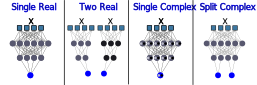
\includegraphics[width=1\textwidth]{./experiments/ground-state-search/ansatz/ansatz.pdf}}
    \caption{
        Schematic visualization of how the four different possibilities for the ansatz are implemented.
        \emph{Single Real} gives a pure real wavefunction output. The architecture is a single network with only real parameters.
        \emph{Two Real} gives a complex wavefunction output (two real numbers, one for the phase and one for the amplitude). The architecture consists of two half-size networks with only real parameters. They do not interact.
        \emph{Single Complex} gives a complex wavefunction output (directly one complex type number). The architecture is a single network with every parameter being a complex number.
        \emph{Split Complex} gives a complex wavefunction output (two real numbers, one for the phase and one for the amplitude). The architecture is a single network with only real parameters, but at the last stage it is split to give two outputs instead of one. The difference to the two real ansatz is that the two \glqq halves\grqq{} of the network can interact.
    }
    \label{fig:ansatz-comparisons}
    
    \makebox[\textwidth][c]{\includegraphics[width=1.1\textwidth]{./experiments/ground-state-search/ansatz/hyperparameter-matrix/hyperparameter-matrix.pdf}}
    \caption{Comparison of hyperparameter combinations. 
            The ansatz is encoded in the dash type, the color specifies the metaformer hyperparameters.
            \emph{sr d:1 e:8} meaning \emph{single real}, \emph{depth 1} and \emph{embed dimension 8}.
            All datasets have been calculated for a randomly encoded \emph{trigonal\_square} lattice with 64 lattice sites.
            Every model is of the type \emph{GPF-NNN} with a mlp-ratio of 4. The Ising parameters are $J=-1$ and $h=-0.7$.
    }
    \label{fig:hyperparameter-matrix}
\end{figure}

        \FloatBarrier
        \subsection{Choice of Hyperparameters}
        \label{sec:experiments-hyperparameters}
        Like mentioned, \autoref{fig:hyperparameter-matrix} compares not only different choices for the network ansatz, but also different hyperparameter combinations.
In general, the behavior of a GPF-NNN on a trigonal\_square lattice is observed.

Many different correlations could be extracted when discussing the graph.
But the obtained relations could not be guaranteed to generalize to different lattice shapes or different Ising parameters.
Because of that, a detailed analysis of the figure would not be very helpful.

Therefore only two clear trends will be mentioned:

First, it can be observed that all combinations of \emph{ansatz}, \emph{depth} and \emph{embed dimension} converge to the same energy (they also have their variance converging in the same order of magnitude, but that data is not pictured in the thesis).
This underlines the robustness of the metaformer architecture.
As all combinations seemingly are a valid parameterization of the wavefunction, it is possible to select the one with the most appropriate performance behavior for the task.

Second, the shallow networks (depth of one, in \autoref{fig:hyperparameter-matrix} red and green) seem to perform best in this task.
In image classification tasks the general rule was established, that while deeper networks are generally harder to train, they perform usually better if successfully trained.
An only one block deep metaformer on the other hand can probably be described as the opposite of a \emph{deep network}.
While the good performance of shallow networks can have multiple reasons, a likely one is the problem's overall difficulty.
In this thesis it was hinted multiple times, that the presented lattices are not \emph{irregular} enough to justify really deep networks.
More \glqq complicated\grqq{} lattice structures or Ising problems might be required to take full advantage of the metaformer's strengths. 
The last section will pick up this thought.

        \FloatBarrier
        \subsection{Differences across the Phase Diagram}
        \label{sec:experiments-phasecriticalpoint}
        The same quantum mechanical system can have different states that are described by wavefunctions of different complexity.
An example might be the behavior of a system as it approaches a specific temperature.
This could be the \emph{boiling point} of a fluid, at which the liquid turns into steam and starts behaving completely differently.
It could also be the approach to \emph{absolute zero}, that is commonly known to be responsible to induce unique behavior in quantum objects.
Depending on the nature of the system, the approach to such a point could make the wavefunction simpler or more difficult to parameterize.

Temperature is not the only parameter that could induce a transition, which is generally known as a \emph{phase transition}.
In our case the \emph{strength of the transverse electromagnetic field} can also cause such a phase transition.

The location of the transition is dictated by the ratio of the Ising parameters $J$ and $h$, $\lambda = \frac{h}{J}$, as well as the shape and dimensionality of the lattice.
The experiments in the preceding sections all used a $\lambda = \frac{h=-0.7}{J=-1} = 0.7$.
In the book \emph{Quantum Ising Phases and Transitions in Transverse Ising Models} \cite{isingBook}, the transverse field Ising phase transition is said to occur around $\lambda = $ \SIrange[]{2}{4}{} for 2D latices of square nature.

Experiments with a CNN around the region of $J = -1$, $h = -3.6$ have shown a significantly larger minimum variance of around \SI[]{0.3}[]{}. 
Compared to the experiments in the past sections this is larger by several orders of magnitude.
Bringing the $h$ parameter closer to zero, made the minimum variance drop quickly ($\approx 0.02$ for $h = -1.7$ down to falling to $< \SI[]{10e-3}[]{}$ for $h = -0.7$, where the computation was stopped after 70 steps).

The reason for operating close to the phase transition region is the increased complexity of the wavefunction.
Previous sections suggested, that the metaformer architecture might be too \glqq complex\grqq{} to represent the basic wavefunctions around $\lambda = 0.7$. 
This might be the reason, why the extremely simple CNN is outperforming the sophisticated metaformer in these examples.

It would be interesting to know, whether the metaformer can describe the complex wavefunctions for larger $\lambda$ better than e.g. a CNN.

While this might be the case, it also might not be.
During experiments on this question, for some runs a better performance was achieved. 
Other runs saw the metaformer or both models crashing due to \emph{NaN} errors after only a few steps.

As presenting a case, in that the metaformer happened to perform better than the CNN would correspond to severe cherry picking, it was decided against it.
Though the exploration of the phase transition region provides an excellent opportunity for further research in this domain.

        \FloatBarrier

\chapter{Conclusion}
\label{sec:conclusion}

% ! Addendum
\input{bibliography}
\chapter{Appendix}
\label{sec:appendix}

%! needs to be first, because of format adapted to chapter title of appendix
\section{Lattice Visualization} \label{appendix:lattice-visualisation}

\begin{minipage}{\linewidth}
    \centering
    \makebox[\textwidth][c]{
        \makebox[1.25\textwidth][c]{
            \makebox[0.40\textwidth][l]{\includegraphics[width=0.33\textwidth]{./../appendix/lattice_visualization/cubic,size=2,np.pdf}}
            \makebox[0.40\textwidth][l]{\includegraphics[width=0.33\textwidth]{./../appendix/lattice_visualization/cubic,size=3,p.pdf}}
            \makebox[0.40\textwidth][l]{\includegraphics[width=0.33\textwidth]{./../appendix/lattice_visualization/cubic,size=4,np.pdf}}
        }
    }

    \captionof{figure}{A visualization of the \textbf{2D-cubic} lattice structure, measured in this thesis. 
        The lattices from left to right can be described by the parameters\\
        1: \emph{size=2, non-periodic}\,\,\,\, 2: \emph{size=3, periodic}\,\,\,\, 3: \emph{size=4, non-periodic}
    }
    \label{fig:appendix-cubic-lattices}
\end{minipage}

\vspace{0.5cm}

\begin{minipage}{\linewidth}
    \centering
    \makebox[\textwidth][c]{
        \makebox[1.25\textwidth][c]{
            \makebox[0.40\textwidth][l]{\includegraphics[width=0.33\textwidth]{./../appendix/lattice_visualization/hexagonal,size=1,np.pdf}}
            \makebox[0.40\textwidth][l]{\includegraphics[width=0.33\textwidth]{./../appendix/lattice_visualization/hexagonal,size=2,np.pdf}}
            \makebox[0.40\textwidth][l]{\includegraphics[width=0.33\textwidth]{./../appendix/lattice_visualization/hexagonal,size=3,p.pdf}}
        }
    }

    \vspace{0.3cm}
    \captionof{figure}{A visualization of the \textbf{2D-hexagonal} lattice structure, measured in this thesis. 
        The lattices from left to right can be described by the parameters \\
        1: \emph{size=1, non-periodic}\,\,\,\, 2: \emph{size=2, non-periodic}\,\,\,\, 3: \emph{size=3, periodic}
    }
    \label{fig:appendix-hexagonal-lattices}
\end{minipage}

\vspace{0.4cm}

\begin{minipage}{\linewidth}
    \centering
    \makebox[\textwidth][c]{
        \makebox[1.25\textwidth][c]{
            \makebox[0.40\textwidth][l]{\includegraphics[width=0.33\textwidth]{./../appendix/lattice_visualization/trigonal_hexagonal,size=1,np.pdf}}
            \makebox[0.40\textwidth][l]{\includegraphics[width=0.33\textwidth]{./../appendix/lattice_visualization/trigonal_hexagonal,size=2,np.pdf}}
            \makebox[0.40\textwidth][l]{\includegraphics[width=0.33\textwidth]{./../appendix/lattice_visualization/trigonal_hexagonal,size=3,p.pdf}}
        }
    }
    
    \vspace{0.5cm}
    \captionof{figure}{A visualization of the \textbf{2D-trigonal\_hexagonal} lattice structure, measured in this thesis. 
        The lattices from left to right can be described by the parameters \\
        1: \emph{size=1, non-periodic}\,\,\,\, 2: \emph{size=2, non-periodic}\,\,\,\, 3: \emph{size=3, periodic}
    }
    \label{fig:appendix-trigonal_hexagonal-lattices}
\end{minipage}

% HERE SHOULD THE PAGE-BREAK BE. i love latex, but stuff like this infuriates me to get correct
\newpage
\makebox{\vspace{5cm}}\\

\begin{minipage}{\linewidth}
    \centering
    \makebox[\textwidth][c]{
        \makebox[1.25\textwidth][c]{
            \makebox[0.40\textwidth][l]{\includegraphics[width=0.33\textwidth]{./../appendix/lattice_visualization/trigonal_square,size=2,np.pdf}}
            \makebox[0.40\textwidth][l]{\includegraphics[width=0.33\textwidth]{./../appendix/lattice_visualization/trigonal_square,size=3,np.pdf}}
            \makebox[0.40\textwidth][l]{\includegraphics[width=0.33\textwidth]{./../appendix/lattice_visualization/trigonal_square,size=4,p.pdf}}
        }
    }

    \vspace{0.4cm}
    \captionof{figure}{A visualization of the \textbf{2D-trigonal\_square} lattice structure, measured in this thesis. 
        The lattices from left to right can be described by the parameters \\
        1: \emph{size=2, non-periodic}\,\,\,\, 2: \emph{size=3, non-periodic}\,\,\,\, 3: \emph{size=4, periodic}
    }
    \label{fig:appendix-trigonal_square-lattices}
\end{minipage}

\vspace{1.2cm}

\begin{minipage}{\linewidth}
    \centering
    \makebox[\textwidth][c]{
        \makebox[1.25\textwidth][c]{
            \makebox[0.40\textwidth][c]{\includegraphics[width=0.20\textwidth]{./../appendix/lattice_visualization/trigonal_diamond,size=3,np.pdf}}
            \makebox[0.40\textwidth][c]{\includegraphics[width=0.20\textwidth]{./../appendix/lattice_visualization/trigonal_diamond,size=4,p.pdf}}
            \makebox[0.40\textwidth][c]{\includegraphics[width=0.20\textwidth]{./../appendix/lattice_visualization/trigonal_diamond,size=5,np.pdf}}
        }
    }

    \vspace{0.4cm}
    \captionof{figure}{A visualization of the \textbf{2D-trigonal\_diamond} lattice structure, measured in this thesis. 
        The lattices from left to right can be described by the parameters \\
        1: \emph{size=3, non-periodic}\,\,\,\, 2: \emph{size=4, periodic}\,\,\,\, 3: \emph{size=5, non-periodic}
    }
    \label{fig:appendix-trigonal_diamond-lattices}
\end{minipage}

\vspace{1.2cm}

\begin{minipage}{\linewidth}
    \centering
    \makebox[\textwidth][c]{\includegraphics[width=0.80\textwidth]{./../appendix/lattice_visualization/linear,size=5,np.pdf}}
    \vspace*{0.2cm}
    \makebox[\textwidth][c]{\includegraphics[width=0.80\textwidth]{./../appendix/lattice_visualization/linear,size=6,p.pdf}}
    \vspace*{0.2cm}
    \makebox[\textwidth][c]{\includegraphics[width=0.80\textwidth]{./../appendix/lattice_visualization/linear,size=8,np.pdf}}

    \vspace{0.2cm}
    \captionof{figure}{A visualization of the \textbf{1D-linear} lattice structure, measured in this thesis. 
        The lattices from top to bottom can be described by the parameters \\
        1: \emph{size=5, non-periodic}\,\,\,\, 2: \emph{size=6, periodic}\,\,\,\, 3: \emph{size=8, non-periodic}
    }
    \label{fig:appendix-linear-lattices}
\end{minipage}

\newpage

% pdf as a additional information, can be nicely ref-ed ("\fullpage{anhang:test}") because of fake section that doesn't get shown in the table of contents
% \includepdf[pagecommand={\section*{} \label{appendix:test}}]{appendix/test.pdf}

% minted to properly import and style code. ! Needs python libraries
\newpage
\section{Dot Product Self Attention (jax)} \label{appendix:attention}
    \cite{selfPhysics}, \filepath{/models/metaformer.py}
    \inputminted[firstline=149, lastline=169]{python}{./../physics-code/models/metaformer.py}

\section{Graph Conformer Module (jax)} \label{appendix:graph-conformer}
    \cite{selfPhysics}, \filepath{/models/metaformer.py}
    \inputminted[firstline=242, lastline=284]{python}{./../physics-code/models/metaformer.py}

\newpage
\section{Graph Poolformer Module (jax)} \label{appendix:graph-poolformer}
    \cite{selfPhysics}, \filepath{/models/metaformer.py}
    \inputminted[firstline=211, lastline=239]{python}{./../physics-code/models/metaformer.py}
    

\end{document}





